\section{Overbelægning}

\subsection{Udvikling og betydning af overbelægning}
Definitionen af overbelægning er en overskridelse af indlagte patienter på en given afdeling ift. tilgængelige sengepladser. Overbelægning er estimeret til at være 85\% af det samlede antal sengepladser, herefter er det påvist at sandsynligheden for hospitalets mortalitet stiger 9\% sammenlignet med ved underbelægning.\citep{Madsen2014} Sengepladserne på sygehusene i Danmark er fra 1996 til 2011 blevet reduceret med 30\%, da der ønskes at opnå en kapacitet på 100\%. 
\citep{Madsen2014}. Et studie beskriver dog at denne reduktion ikke nødvendigvis har en betydning for mortaliteten, men kan være et tegn på effektivisering af sygehusene. \citep{Madsen2014}

\begin{figure}[H]
\centering
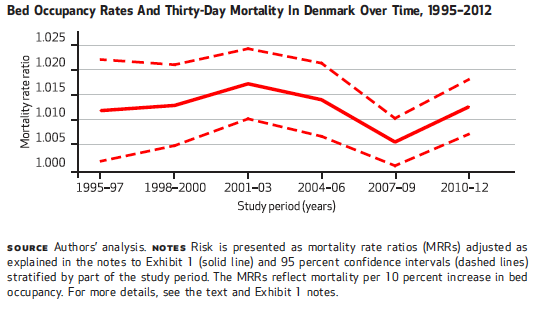
\includegraphics[width=1\textwidth]{figures/overbelaegning_graf.fig}
\caption{sengebelægningsprocent og tredive-dages dødeligheden i Danmark over tid fra 1995-2012}
\label{fig:overbelaegning_graf}
\end{figure}

\noindent
Det fremgår af \autoref{fig:overbelaegning_graf} at der er en begyndende stigning i mortaliteten sammenlignet med sengebelægningsprocenten fra år 2009 og frem.... SKRIV MERE HER...
\citep{dodlighed2014} For at mindske konsekvenser af dette er det vigtigt at finde en ligevægt mellem over- og underbelægning.  


\subsection{Overbelægning i Danmark}
Antallet af patienter, der indlægges varierer fra måned til måned, hvorfor tilgængeligheden af sengepladser også variererer. Dette gør sig gældende på flere forskellige afdelinger i Danmark, hvilket er illustreret på \autoref{fig:overbelaegning_ran}.
                   
\begin{figure}[H]
\centering
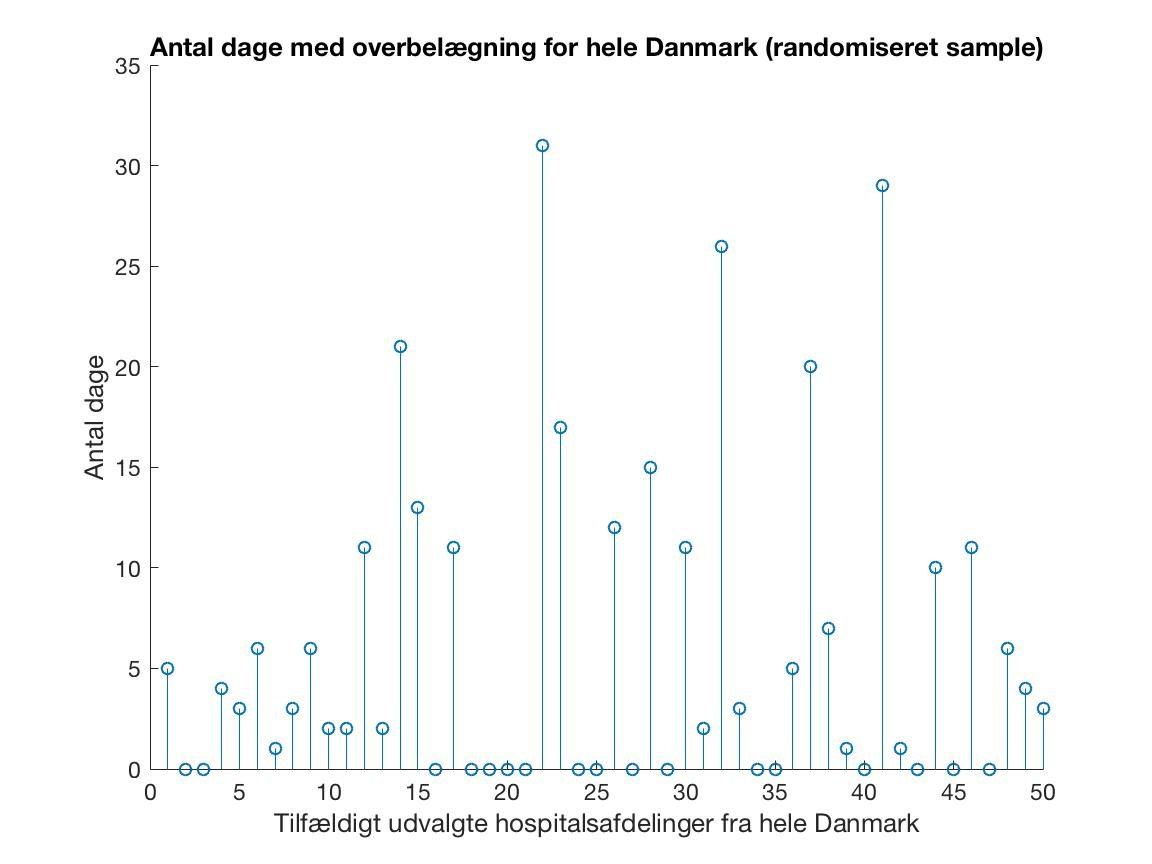
\includegraphics[width=1\textwidth]{figures/overbelaegning_ran.fig}
\caption{Antal dage med overbelægning udarbejdet med tilfældig udvalgte hospitalsafdelinger fra hele Danmark. De randomiserede data er taget over en periode på 6 måneder fra januar til juni i år 2015. \citep{SDS2015}}
\label{fig:overbelaegning_ran}
\end{figure}

\noindent
Det ses udfra ovenstående figur, at der er en tendens til overbelægning på flere hospitalsafdelinger i Danmark i forhold til underbelægning. Overbelægning strækker sig op til en måned. Det fremgår yderligere at der er en uligvægt mellem over- og underbelægning på de enkelte afdelinger. I de måneder hvor overbelægningen er størst, hvilket er januar til marts er overbelægningen på over 5 dage. Hvis der tages udgangspunkt i en enkelt afdeling understøttes det at der er et skel mellem over- og underbelægning.\citep{SDS2015}      

\begin{figure}[H]
\centering
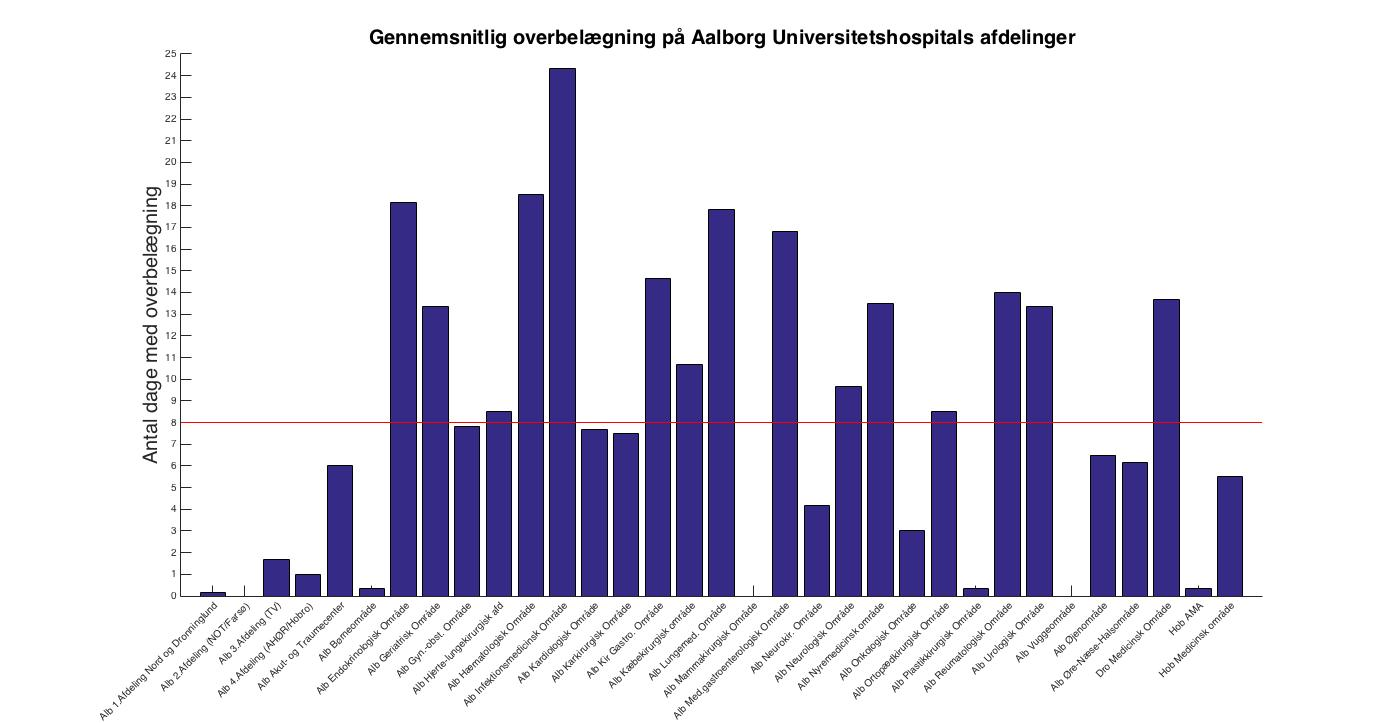
\includegraphics[width=1\textwidth]{figures/overbelaegning_AUH.fig}
\caption{Gennemsnitlig overbelægning på Aalborg Universitetshospitals afdelinger målt i antal dage. Målingerne er taget for samtlige afdelinger på Aalborg Universitetshospital og er taget over en periode på 6 måeneder fra januar til juni i år 2015.\citep{SDS2015}}
\label{fig:overbelaegning_AUH}
\end{figure}

\noindent
Det fremgår af \autoref{fig:overbelaegning_AUH} at den gennemsnitlige overbelægning på Aalborg Universitetshospital strækker sig op til 24 dage og at forholdet mellem over- og underbelægning variererer. Overbelægninger er størst på ambulatorisk infektionsmedicinsk område, ambulatorisk hæmatologisk område og ambulatorisk endokirinologisk. Det fremgår yderligere at der ingen overbelægninger er på ambulatorisk 2. afdeling, ambulatorisk mammakirugisk  område og ambulatorisk vuggeområde. Det ses desuden, at den gennemsnitlige overbelægning på samtlige afdelinger vare optil 8 dage. Det fremgår ligledes for Aalborg universitetshospital at overbelægningen er et større problem i perioden fra januar til marts med en overbelægning på 10 dage \citep{SDS2015}.    





